\subsection{Opportunistic Charging}
\label{subsec-opportunistic}

\begin{figure}[t]
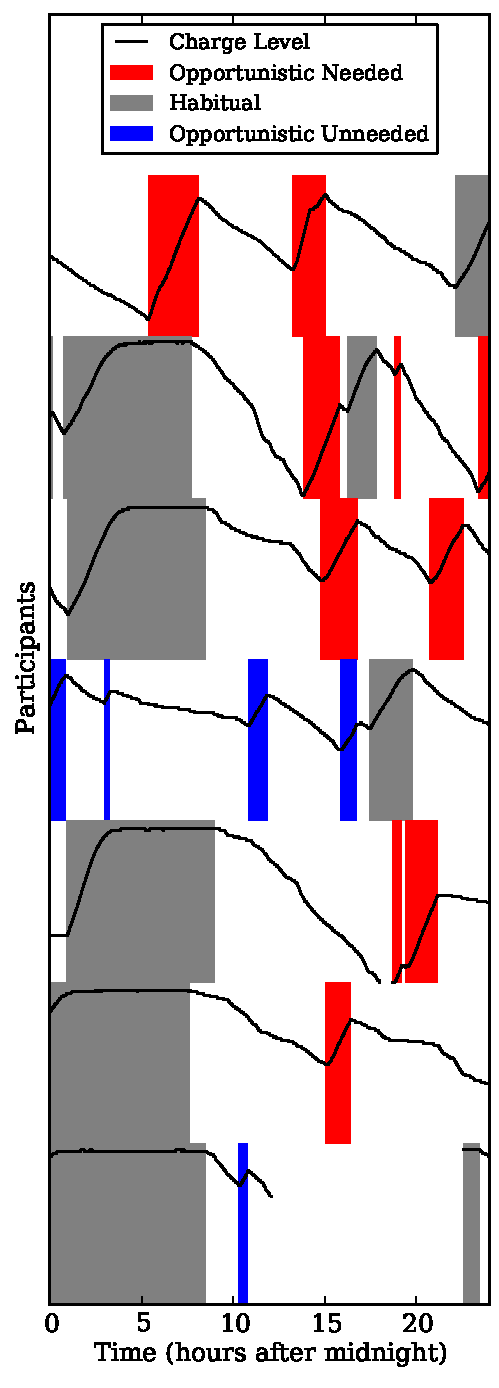
\includegraphics[width=\columnwidth]{./figures/power/opportunistic_charging/count_and_by_time/graph.pdf}
\caption{Patterns of opportunistic charging.}
\end{figure}

One way that users work around the battery limitations of their smartphone
devices is by finding new times and places to charge their phones during the
day: plugging in at their desk at work, in the car during their commute, or
at home before a long night out. We refer to these charging sessions as
opportunistic to distinguish them from more habitual nightly charging.
Assuming that many smartphone users encounter plug points throughout the day,
engaging in opportunistic charging becomes an additional sign of energy
awareness, and understanding opportunistic charging becomes necessary to
improving energy management on mobile devices.

\subsubsection{Seizing Energy Opportunities}

\begin{figure*}[t]
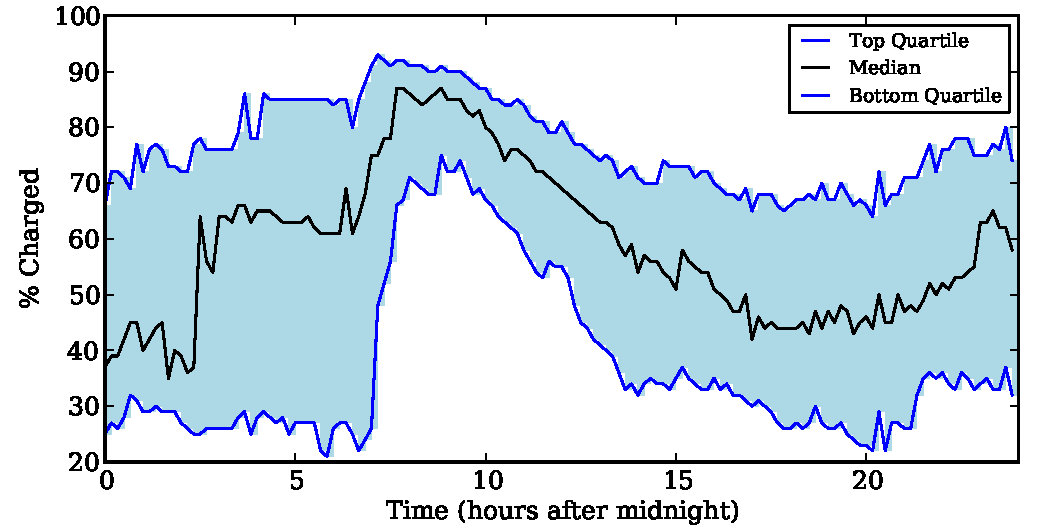
\includegraphics[width=\textwidth]{./figures/power/opportunistic_charging/max_difference/graph.pdf}
\caption{Charge difference between participants during one day.
\textnormal{The graph plots the top and bottom quartiles as well as the
median. A significant spread is present on the testbed throughout the day,
making charging sharing protocols possible.}}
\end{figure*}

\subsubsection{Future Experiments}

% \cite{banerjee:ubicomp:2007, rahmati:mobilehci:2007}
